\subsection{Elektroninė metalų laidumo teorija}

Metaluose krūvio nešėjai yra elektronai. Pagrindimas: 

Elektronas, susidūręs su metalo gardelės jonu, gali pradėti judėti
bet kuria kryptimi ir po kiekvieno tokio susidūrimo dreifuojančio
elektrono pradinis greitis yra lygus nuliui. Dėl elektrinio lauko
poveikio, elektronas pradeda judėti jo veikimo kryptimi ir per laiką
$t$ vėl sutinka gardelės joną.

Elektrono inercijos jėga:
\begin{equation*}
  F_{\t{in}} = -ma
\end{equation*}
čia:
\begin{description}
  \item[$m$] – masė;
  \item[$a$] – pagreitis.
\end{description}

Elektros šaltinio kuriama elektros varomoji jėga:
\begin{align}
  E &= \frac{A_{\t{paš}}}{q} \\
  \intertext{Kadangi darbas yra lygus jėgos ir kelio sandaugai:}
  &= \frac{F_{\t{in}} l}{q} \\
  &= -\frac{mal}{q} \\
  \intertext{Pagal apibrėžimą, pagreitis yra greičio pokytis per laiko
  vienetą. Kadangi, pas mus pradinis greitis yra 0, tai gauname:}
  &= -\frac{mvl}{qt} \label{eq:metalu_laidumo_1} \\
\end{align}
čia:
\begin{description}
  \item[$A_{\t{paš}}$] – pašalinių jėgų darbas;
  \item[$q$] – pratekėjęs krūvis;
  \item[$F_{\t{in}}$] – inercijos jėga;
  \item[$l$] – laidininko ilgis.
  \item[$v$] – elektrono per laiką $t$ pasiektas greitis;
  \item[$t$] – po kiek laiko nuo judėjimo pradžios elektronas sutiko
    joną.
\end{description}

Krūvis, kuris prateka laidininku:
\begin{equation}
  Q = I t \label{eq:metalu_laidumo_3}
\end{equation}
čia:
\begin{description}
  \item[$I$] – srovės stipris.
\end{description}

Iš Omo dėsnio:
\begin{align}
  I &= \frac{E}{R} \\
  \intertext{Įsistatome \ref{eq:metalu_laidumo_1} ir gauname:}
  &= -\frac{mal}{Rq} \label{eq:metalu_laidumo_2} \\
\end{align}
čia:
\begin{description}
  \item[$R$] – laidininkų ir galvanometro varža.
\end{description}

Sulyginę \ref{eq:metalu_laidumo_2} ir \ref{eq:metalu_laidumo_3}
gauname:
\begin{align*}
  I &= \frac{mlv_{0}}{qRt} \\
  &= \frac{Q}{t} \\
  \frac{q}{m}
  &= \frac{v_{0}l}{QR} \\
  &= (\t{nuo }1,5 \t{ iki } 1,6) \cdot 10^{11} \tfrac{C}{kg}
\end{align*}
čia:
\begin{description}
  \item[$\frac{q}{m}$] – savitasis dalelės krūvis.
\end{description}

Gautąjį savitąjį dalelės krūvį palyginę su elektrono:
\begin{align*}
  \frac{e}{m} &= 1,76 \cdot 10^{11} \tfrac{C}{kg}.
\end{align*}
galime teigti, jog krūvio nešėjai yra elektronai.

TODO: Suprasti ir perrašyti.

\begin{align*}
  \frac{mv^{2}}{2} &= \frac{3}{2} k T
\end{align*}

\begin{align*}
  v_{kv} &= 1,1 \cdot 10^{5} \tfrac{m}{s}
\end{align*}

Tvarkingo judėjimo greitis:
\begin{align*}
  v &\equiv 8 \cdot 10^{-4} \tfrac{m}{s}
\end{align*}

Vidutinis elektrono greitis (?):
\begin{align*}
  \t{ū} &= 10^{6} \tfrac{m}{s}
\end{align*}

Elektrono greitis:
\begin{align*}
  v &= \mu E
\end{align*}

\section{Magnetinis laukas}

\subsection{Srovės magnetinis laukas}

\begin{defn}[Magnetinis laukas]
  Ypatingos formos materija, perduodanti judančių elektros krūvių
  sąveiką.
\end{defn}

\begin{defn}[Magnetinio lauko stipris]
  Dydis apibūdinantis magnetinio lauko stiprumą vakuume.
  \begin{equation*}
    H = \frac{I}{l}
  \end{equation*}
  čia:
  \begin{description}
    \item[$\vec{H}$] – magnetinio lauko stipris (matuojamas $\frac{A}{m}$);
    \item[$I$] – srovės stipris;
    \item[$l$] – magnetinės linijos, einančios per duotąjį tašką, ilgis.
  \end{description}
  Magnetinio lauko stiprio vektoriaus kryptis yra išilgai magnetinio
  lauko jėgų linijos liestinės į tą pusę, kurią rodo magnetinės rodyklės
  šiaurės polius.
\end{defn}

\begin{defn}[Magnetinė indukcija]
  Jėginė magnetininio lauko charakteristika. Apibūdina magnetinio lauko
  stiprumą medžiagoje.
  \begin{equation*}
    \vec{B} = \mu_{0} \mu \vec{H}
  \end{equation*}
  čia:
  \begin{description}
    \item[$\vec{B}$] – magnetinė indukcija (matuojama teslomis
      $1T = 1\frac{N}{Am}$);
    \item[$\mu_{0}$] – magnetinė konstanta 
      ($\mu_{0} = 4\pi \cdot 10^{-7} \frac{N}{A^{2}} = 1,25 \cdot 10^{-6} 
      \frac{N}{A^{2}}$);
    \item[$\mu$] – santykinė aplinkos magnetinė skvarba;
    \item[$\vec{H}$] – magnetinio lauko stipris.
  \end{description}
\end{defn}

\begin{defn}[Lorenco jėga]
  Jėga, kuria magnetinis laukas veikia judančią elektringąją dalelę:
  \begin{align*}
    F_{L}
    &= q | \vec{v} \cdot \vec{B}| \\
    &= q v B \sin \alpha \\
  \end{align*}
  čia:
  \begin{description}
    \item[$q$] – dalelės krūvis;
    \item[$\vec{v}$] – dalelės greitis;
    \item[$\vec{B}$] – magnetinės indukcijos vektorius;
    \item[$\alpha$] – kampas tarp $\vec{v}$ ir $\vec{B}$.
  \end{description}
  Lorenco jėga yra statmena $\vec{v}$ ir $\vec{B}$.
  (Žr. \ref{fig:lorenco_jega} paveikslėlį.)
\end{defn}

\begin{figure}[H]
  \begin{center}
    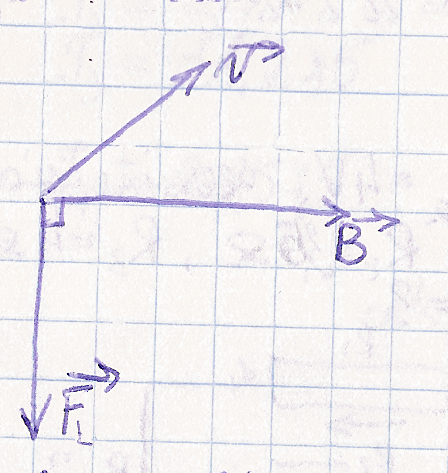
\includegraphics[height=0.5\textwidth]{images/lorenco_jega.png}
  \end{center}
  \caption{Lorenco jėga}
  \label{fig:lorenco_jega}
\end{figure}

\begin{defn}[Ampero jėga]
  Laidininką, kuriuo teka elektros srovė, magnetiniame lauke veikianti
  jėga.

  \begin{equation*}
    F_{A} = I l B \sin \alpha
  \end{equation*}
  čia:
  \begin{description}
    \item[$I$] – laidininku tekančios srovės stipris;
    \item[$l$] – laidininko ilgis;
    \item[$B$] – magnetinė indukcija;
    \item[$\alpha$] – kampas tarp elektros srovės ir magnetinės
      indukcijos krypčių.
  \end{description}
\end{defn}

Elektromagnetiniame lauke judantį krūvį veikianti jėga:
\begin{align*}
  F &= q \vec{E} + q \left[ \vec{v} \cdot \vec{B} \right]
\end{align*}

Suraskime tiesaus begalinio laidininko nuo jo atstumu $r_{0}$ esančiame
taške kuriamą indukciją:
\begin{align*}
  \intertext{nykstamai trumpos laidininko atkarpos kuriama magnetinė
  indukcija:}  
  B
  &= \mu_{0} \mu H \\
  &= \mu_{0} \mu \frac{I}{l} \\
  \intertext{$l$ yra apskritimo, kurio spindulys jungia tašką su 
  nagrinėjama laidininko atkarpa, ilgis:}
  l
  &= 2 \pi r \\
  &= 2 \pi \frac{r_{0}}{\cos \alpha} \\
  \intertext{sujungę gauname:}
  B
  &= \mu_{0} \mu \frac{I \cos \alpha}{2 \pi r_{0}} \\
  \intertext{kadangi mūsų laidininkas yra begalinio ilgio, tai
  $\alpha$ kitimo sritis yra nuo $-\frac{\pi}{2}$ iki $\frac{\pi}{2}$:}
  B
  &= 2 \int _{0} ^{\frac{\pi}{2}} \mu_{0} \mu 
    \frac{I \cos \alpha}{2 \pi r_{0}} d \alpha \\
  &= 2 \mu_{0} \mu \frac{I}{2 \pi r_{0}}
    \int _{0} ^{\frac{\pi}{2}} \cos \alpha d\alpha \\
  &= \frac{\mu_{0} \mu}{\pi} \frac{I}{r_{0}}\\
  \intertext{FIXME: Turėjo gautis:}
  B &= \frac{\mu_{0} \mu}{2 \pi} \frac{I}{r_{0}}
\end{align*}
